\documentclass[a4paper]{article}
\usepackage[T1]{fontenc}
\usepackage[utf8]{inputenc}
\usepackage{lmodern}
\usepackage{graphicx}
\usepackage[left=2.5cm,right=2.5cm,top=3cm,bottom=3cm]{geometry}
\usepackage{eurosym}
\usepackage{fancyhdr}%encabezado y pie de página
\usepackage[colorlinks=true, linkcolor=black, urlcolor=blue]{hyperref}
\setcounter{secnumdepth}{5}
\usepackage[spanish]{babel}
\setcounter{tocdepth}{5}
\usepackage{colortbl}%para colorear tablas
\usepackage{tabularx}
\usepackage{placeins}%para poner barrera y no pasen de secciones los elementos flotantes
%\usepackage{wasysym} %para poner símbolos
\usepackage{bbding} %para poner símbolos



%para el mapa mental
\usepackage{tikz}
\usetikzlibrary{mindmap,trees}
\usepackage{verbatim}


\date{}
\author{D. Ramirez Ambrosi \\ J. I. Sánchez Méndez \\ J. Rodríguez Azpeleta}
\title{\begin{center}
\textbf{\Huge{Make Yourself Strong}} \\ Prototipo digital  \\Proyecto de la asignatura Interacción Persona Computador \\ \Huge{Grupo 10}
\end{center}}
\date{\today}


\pagestyle{fancy}
\rhead{
\textbf{Make Yourself Strong} \hfill \textbf{Fecha:} \date{\today}
}

\lhead{}

%Separación entre párrafos
\setlength{\parskip}{3mm}

%colores
\definecolor{verde}{RGB}{127,255,0}%color para la barra de titulo
\definecolor{rojo}{RGB}{255,0,0}%color para características
\renewcommand\listfigurename{\centering LISTA DE FIGURAS}

\begin{document}
\maketitle

\thispagestyle{empty}%para evitar enumeración de la página de la portada y del índice
\newpage
\tableofcontents%índice
\thispagestyle{empty}
\newpage



%lista de figuras 
%\renewcommand\listfigurename{\centering LISTA DE FIGURAS}
%\listoffigures
%\clearpage

%Lista de tablas
%\renewcommand{\listtablename}{\centering ÍNDICE DE TABLAS} %Para cambiar el índice de las tablas
%\listoftables
%\thispagestyle{empty}
%\newpage

\setcounter{page}{1}%Para reiniciar el contador de páginas en la página deseada


\section{Tareas realizables}

Las tareas implementadas en el \textbf{prototipo digital único} entregado son las presentadas a continuación. El prototipo se ha creado teniendo en cuenta que \textbf{hay un usuario logueado} en el sistema, \textbf{salvo en una} de las funcionalidades, donde se ha sido más conveniente mostrarla como si no lo estuviera:

\begin{itemize}
	\item   \textbf{Añadir un entrenamiento}: en este caso, ya que hay ya un entrenamiento introducido en la fecha indicada, se trata de \textbf{modificar} un entrenamiento. Sin embargo, esto nos sirve para \textbf{mostrar avisos} al estar un entrenamiento registrado y mostrar los datos ya almacenados para su edición. Así mismo, esta función implementa los \textbf{mensajes emergentes de ayuda} en las señales indicadas.
	
	\item   \textbf{Consultar a un experto}: se implementa la interacción propia del \textbf{envío de mensajes a un experto} que el usuario elija. En este caso \textbf{la interacción se ha preparado para un usuario no registrado} en la aplicación, de forma que se vea claramente que éstos usuarios también pueden probar los servicios.
	
	\item   \textbf{Búsqueda de gimnasios}: cualquier usuario puede realizar una búsqueda de sus gimnasios próximos.
	
	\item   \textbf{Obtención de entrenamiento personalizado}: se ha implementado de forma que los usuarios no registrados puedan elegir sus parámetros más adecuados y se muestre el entrenamiento más conveniente.
	
	\item   \textbf{Redacción de un artículo}: se permite acceder a la pantalla de redacción y, tras el ``envío'', mostrar los errores que pudieran darse.
	
	\item   \textbf{Navegación}: se han creado diferentes páginas generales y de la sección personal del usuario de forma que \textbf{se pueda navegar} por las mismas y \textbf{observar los contenidos} disponibles en ellas.
\end{itemize}

\section{Encuesta}
 Para la realización de esta práctica se ha creado una encuesta con el fin de identificar las funciones y apartados de mayor importancia para usuarios potenciales de la aplicación. Con ello, se ha creado una estructuración de menús teniendo en cuenta las opiniones recogidas.
 
 A continuación se incluye la encuesta realizada y, posteriormente, los resultados de la misma.
 
 \subsection{Anexo: encuesta}
 
 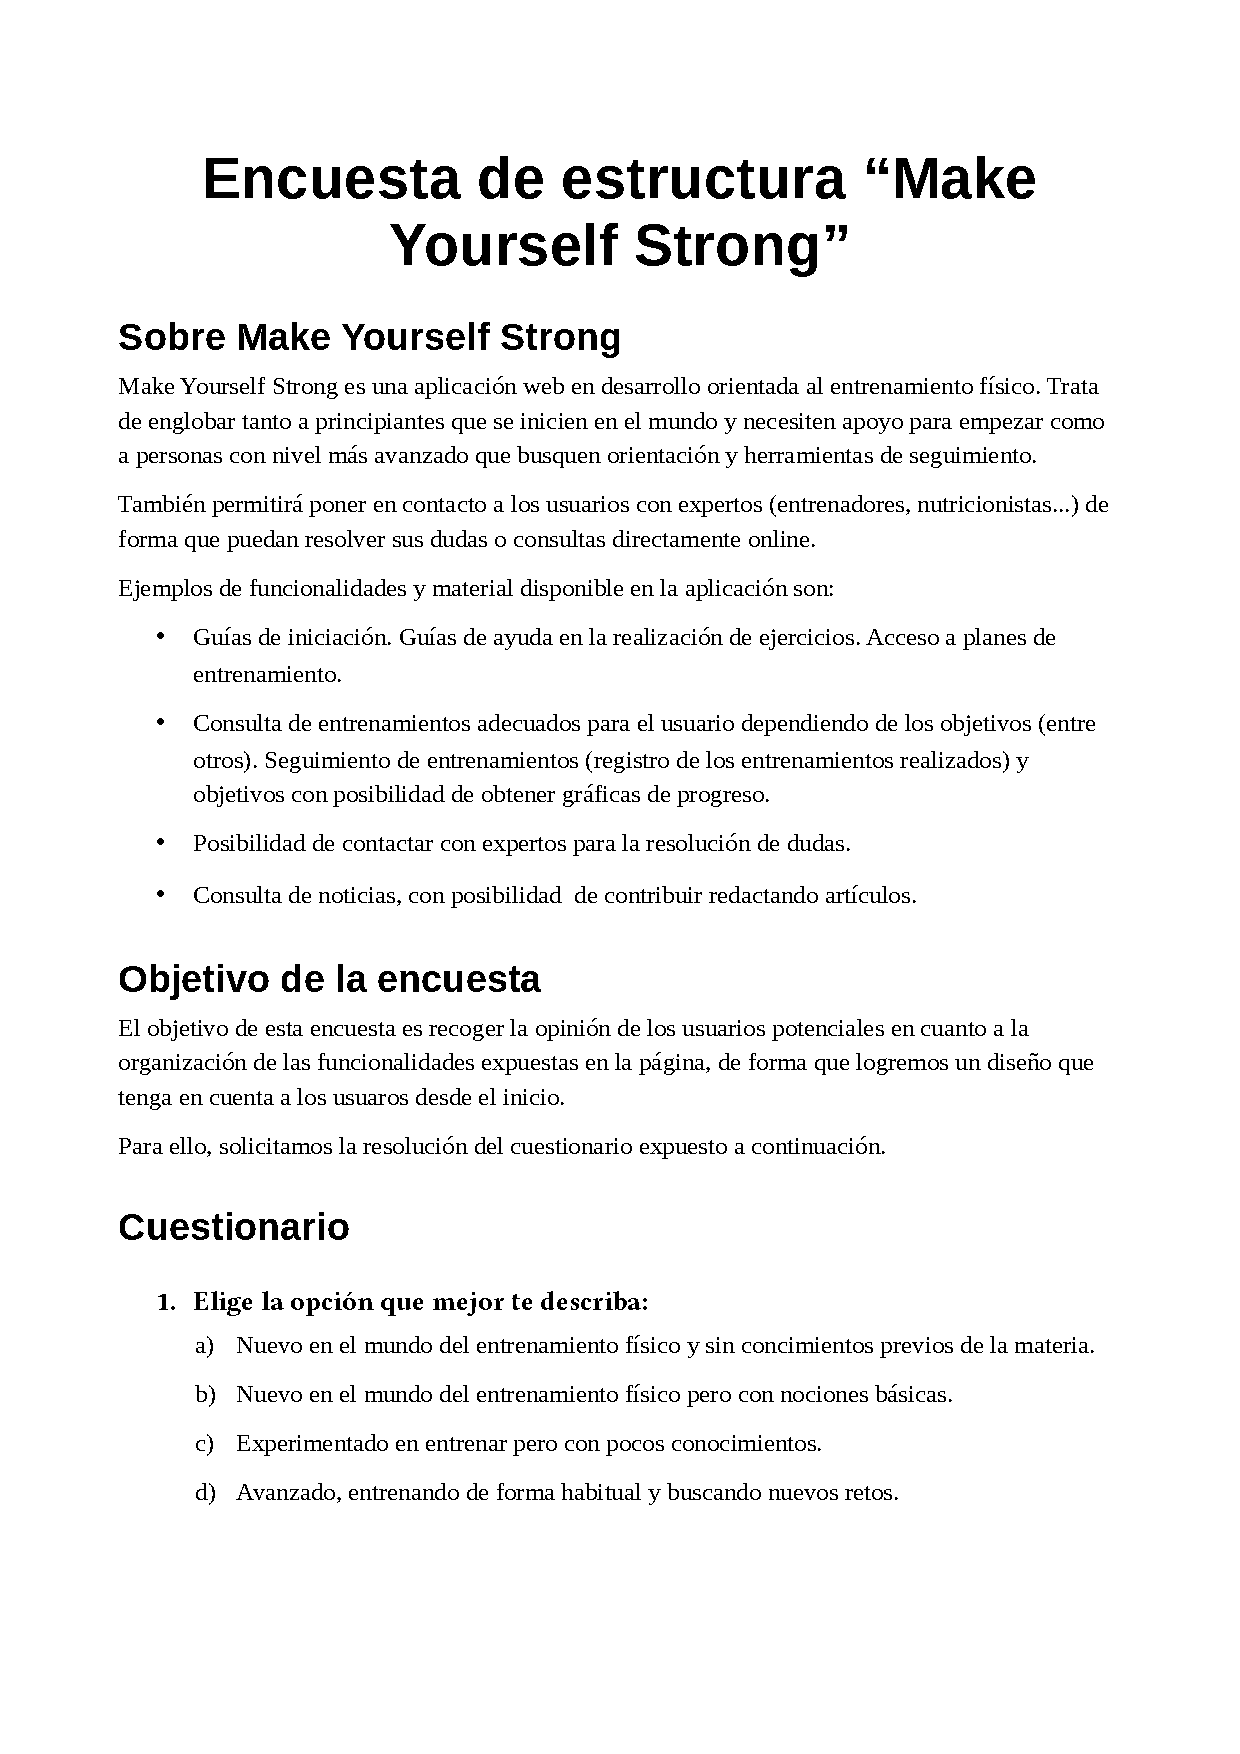
\includegraphics[width=\textwidth, page=1]{./figuras/encuesta.pdf}
 \includegraphics[width=\textwidth, page=2]{./figuras/encuesta.pdf}
 \includegraphics[width=\textwidth, page=3]{./figuras/encuesta.pdf}
 
 \subsection{Resultados de la encuesta}

\begin{figure}[!h]
\centering
 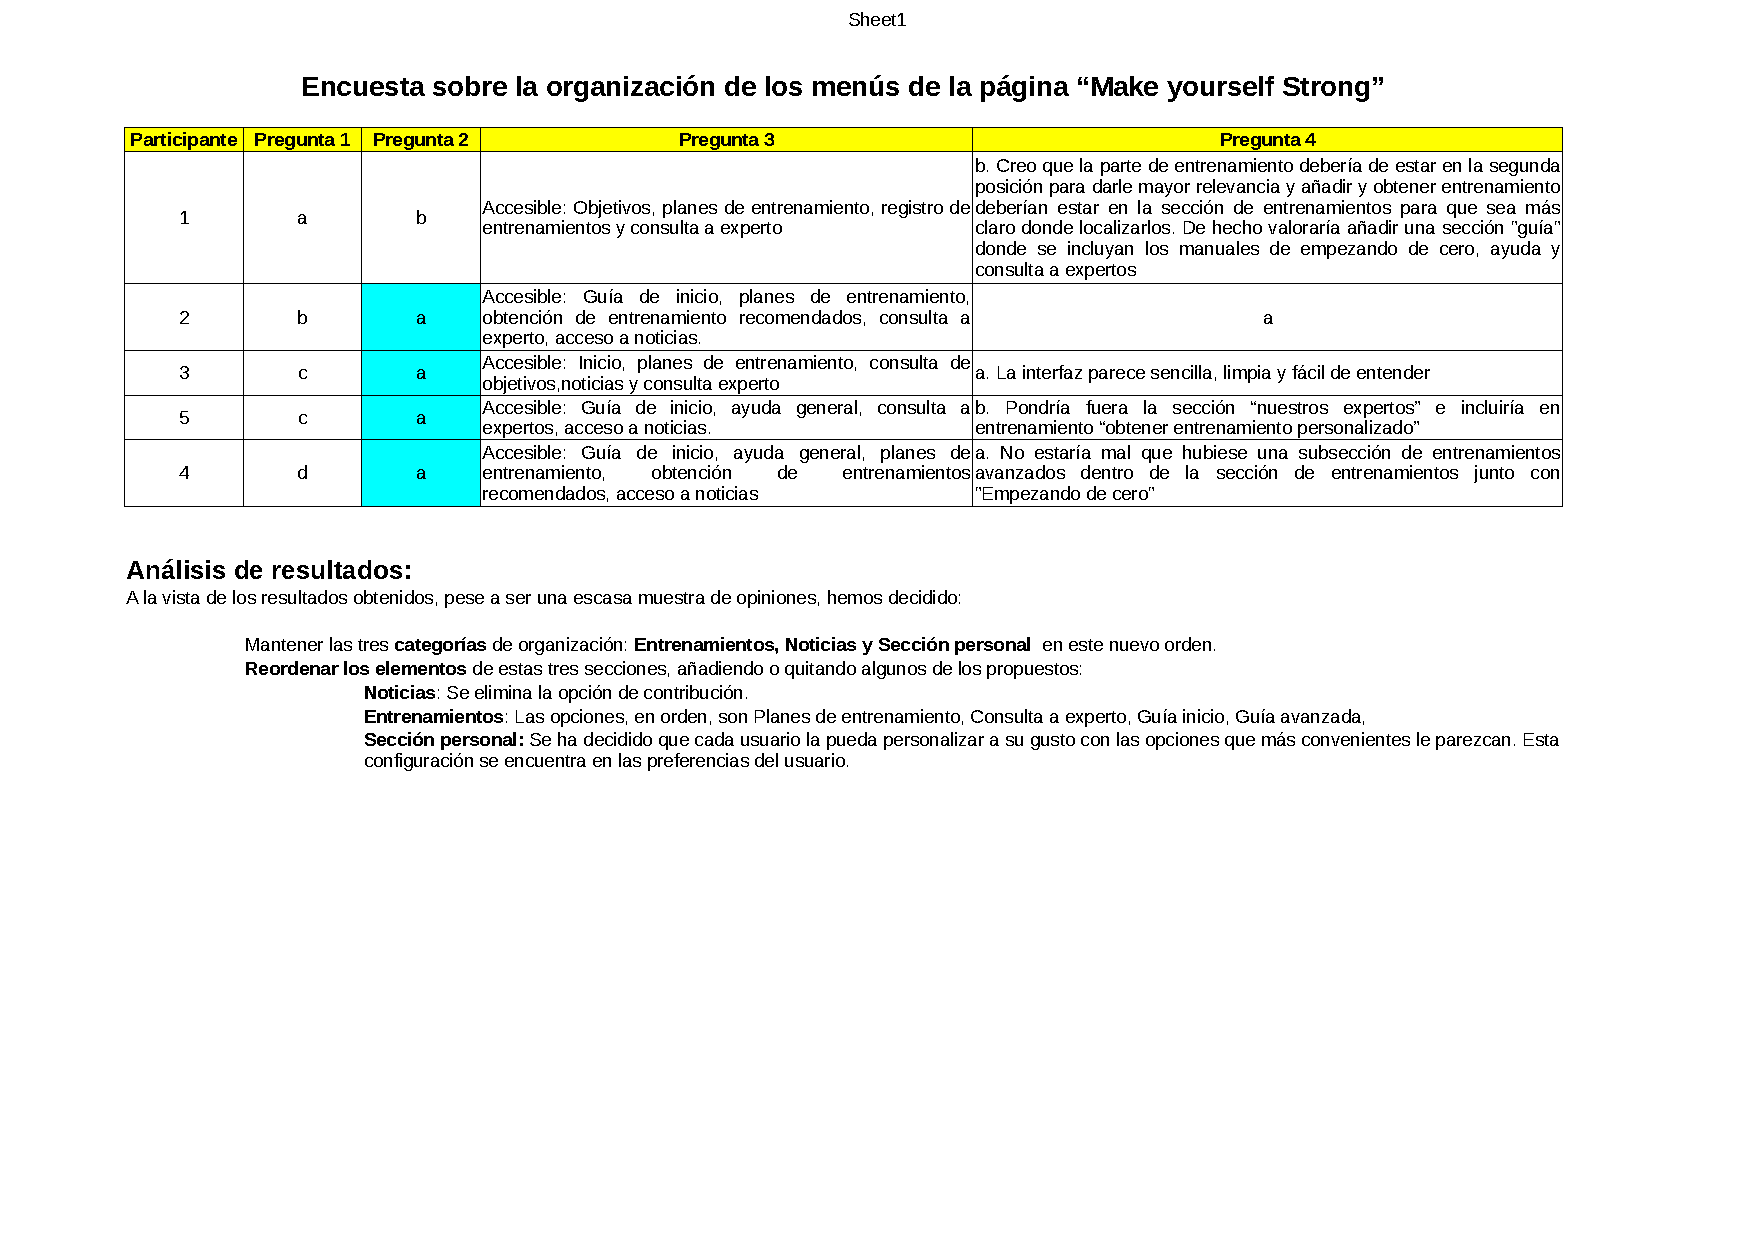
\includegraphics[angle=90,height=0.95\textheight,clip=true,trim=1cm 7cm 2cm 1cm]{./figuras/resultado-encuesta.pdf}
 \end{figure}
 
 
\end{document}